%
% File naaclhlt2013.tex
%

\documentclass[11pt,letterpaper]{article}
\usepackage{naaclhlt2013}
\usepackage{times}
\usepackage{latexsym}
\usepackage{graphicx} % To include figures
\usepackage[titletoc]{appendix}

\setlength\titlebox{6.5cm}    % Expanding the titlebox

\title{Automatic Reviewer: Predicting Whether a Paper will be Accepted or Rejected}

\author{Hong Wang\\
	    Department of Computer Science\\
	    University of Illinois at Chicago\\
	    Chicago, IL 60607, USA\\
	    {\tt hwang207@uic.edu}
	  \And
	Shuyang Lin\\
  	 Department of Computer Science\\
	    University of Illinois at Chicago\\
	    Chicago, IL 60607, USA\\
	  {\tt slin38@uic.edu}}

\date{}

\begin{document}
\maketitle
\begin{abstract}
	//TODO
\end{abstract}

\section{Introduction}
After submitted a paper to a conference, you, as the author of the paper, usually are most interested in whether your paper will be accepted or not.
However, it is the decision made by the reviewers of conference. 
One question rises here is that “can we predict the result?” or more specifically, “can we find the criteria of a certain conference?” 
In this paper, we introduce Automatic Reviewer which may give you the answers, even before you submit the paper to the conference. 

This paper studies the following two problems: 
1. What statistical features of papers are correlated to the decision of the conference? 
2. To what extent can an automatic program predict whether a paper will be accepted or not?

We extract several features which range from paper metadata to paper topics. 
We use supervised learning algorithm (SVM) to learn our system model, and use cross-fold validation to evaluate our method. 

\section{Related Work}

Predicting has been studied in many areas, especially in economics.?? Hal Varian studied using Google queries to help predict economic activity 
%(http://static.googleusercontent.com/external_content/untrusted_dlcp/www.google.com/en/us/googleblogs/pdfs/google_predicting_the_present.pdf)
// TODO more examples??

However, as far as we know, no similar study has been done in predicting conference paper acceptance. The only related study is focus on the visual structure of papers [??]. 

// TODO 4 related papers?!



\section{Data Set}
Currently, we only focus on ACL conference papers. We also limited our study to the papers which were published in year 2007, 2010, and 2012. The reason is that ??
The full papers are used as positive samples. Due to lack of real rejected papers, we assume that all the workshop papers are not as good as the full papers, and use them as negative samples in our study. The statistics of dataset is listed as below: 

We use different features: some of them are directly extracted from the paper; the others are calculated by using several different techniques. 

•	Metadata
Metadata are those information extracted from paper itself, like the number of pages, total numbers of tables/formulas/figures, number of tables/formulas/figures per page, max number of tables/formulas/figures per page. In our current experiment, we only use total number of tables/formulas/figures as features.

•	Author Ranking
We extracted top 2000 authors in “Natural Language \& Speech” area from Microsoft Academic Search [??], and use this extracted list as the authors’ ranking. If author doesn’t appear in the list, the rank will be zero.

•	Popular techniques mentioned in the paper
We also manually created a list of popular techniques which may be used in the NLP research. The terms of techniques and its synonyms are group together. We check each technique in the paper, to see if it has been mentioned or not.

•	Words in the Title (TF-IDF Score)
Based on the assumption that novel ideas are favored in the conference, and such papers may have titles that contain novel terms which are more attractive to the reviewers, we count the TF-IDF score for the title terms, and use score as one of features.

•	Topic – LDA (Latent Dirichlet Allocation )
LDA is used to extract topics from all the papers. In our experiment, top 20 topics are extracted, and the probability distribution vector of topics is used as one feature. 

•	Sentence complexity
All the content sentences within papers are parsed into phrase structure tree by using Stanford Parser [??]. The depth of tree is used as complexity of the corresponding sentence.  //TODO how exactly we use it??


Papers are first parsed into structured data (Java objects). Metadata from the paper are used directly as features. Then the parsed papers are processed by several feature extractors. Finally, the feature vectors are sent to Support Vector Machines (SVM) for model learning and evaluation.


\section{Approaches}
\begin{figure*}[htb]
  \centering
	 	 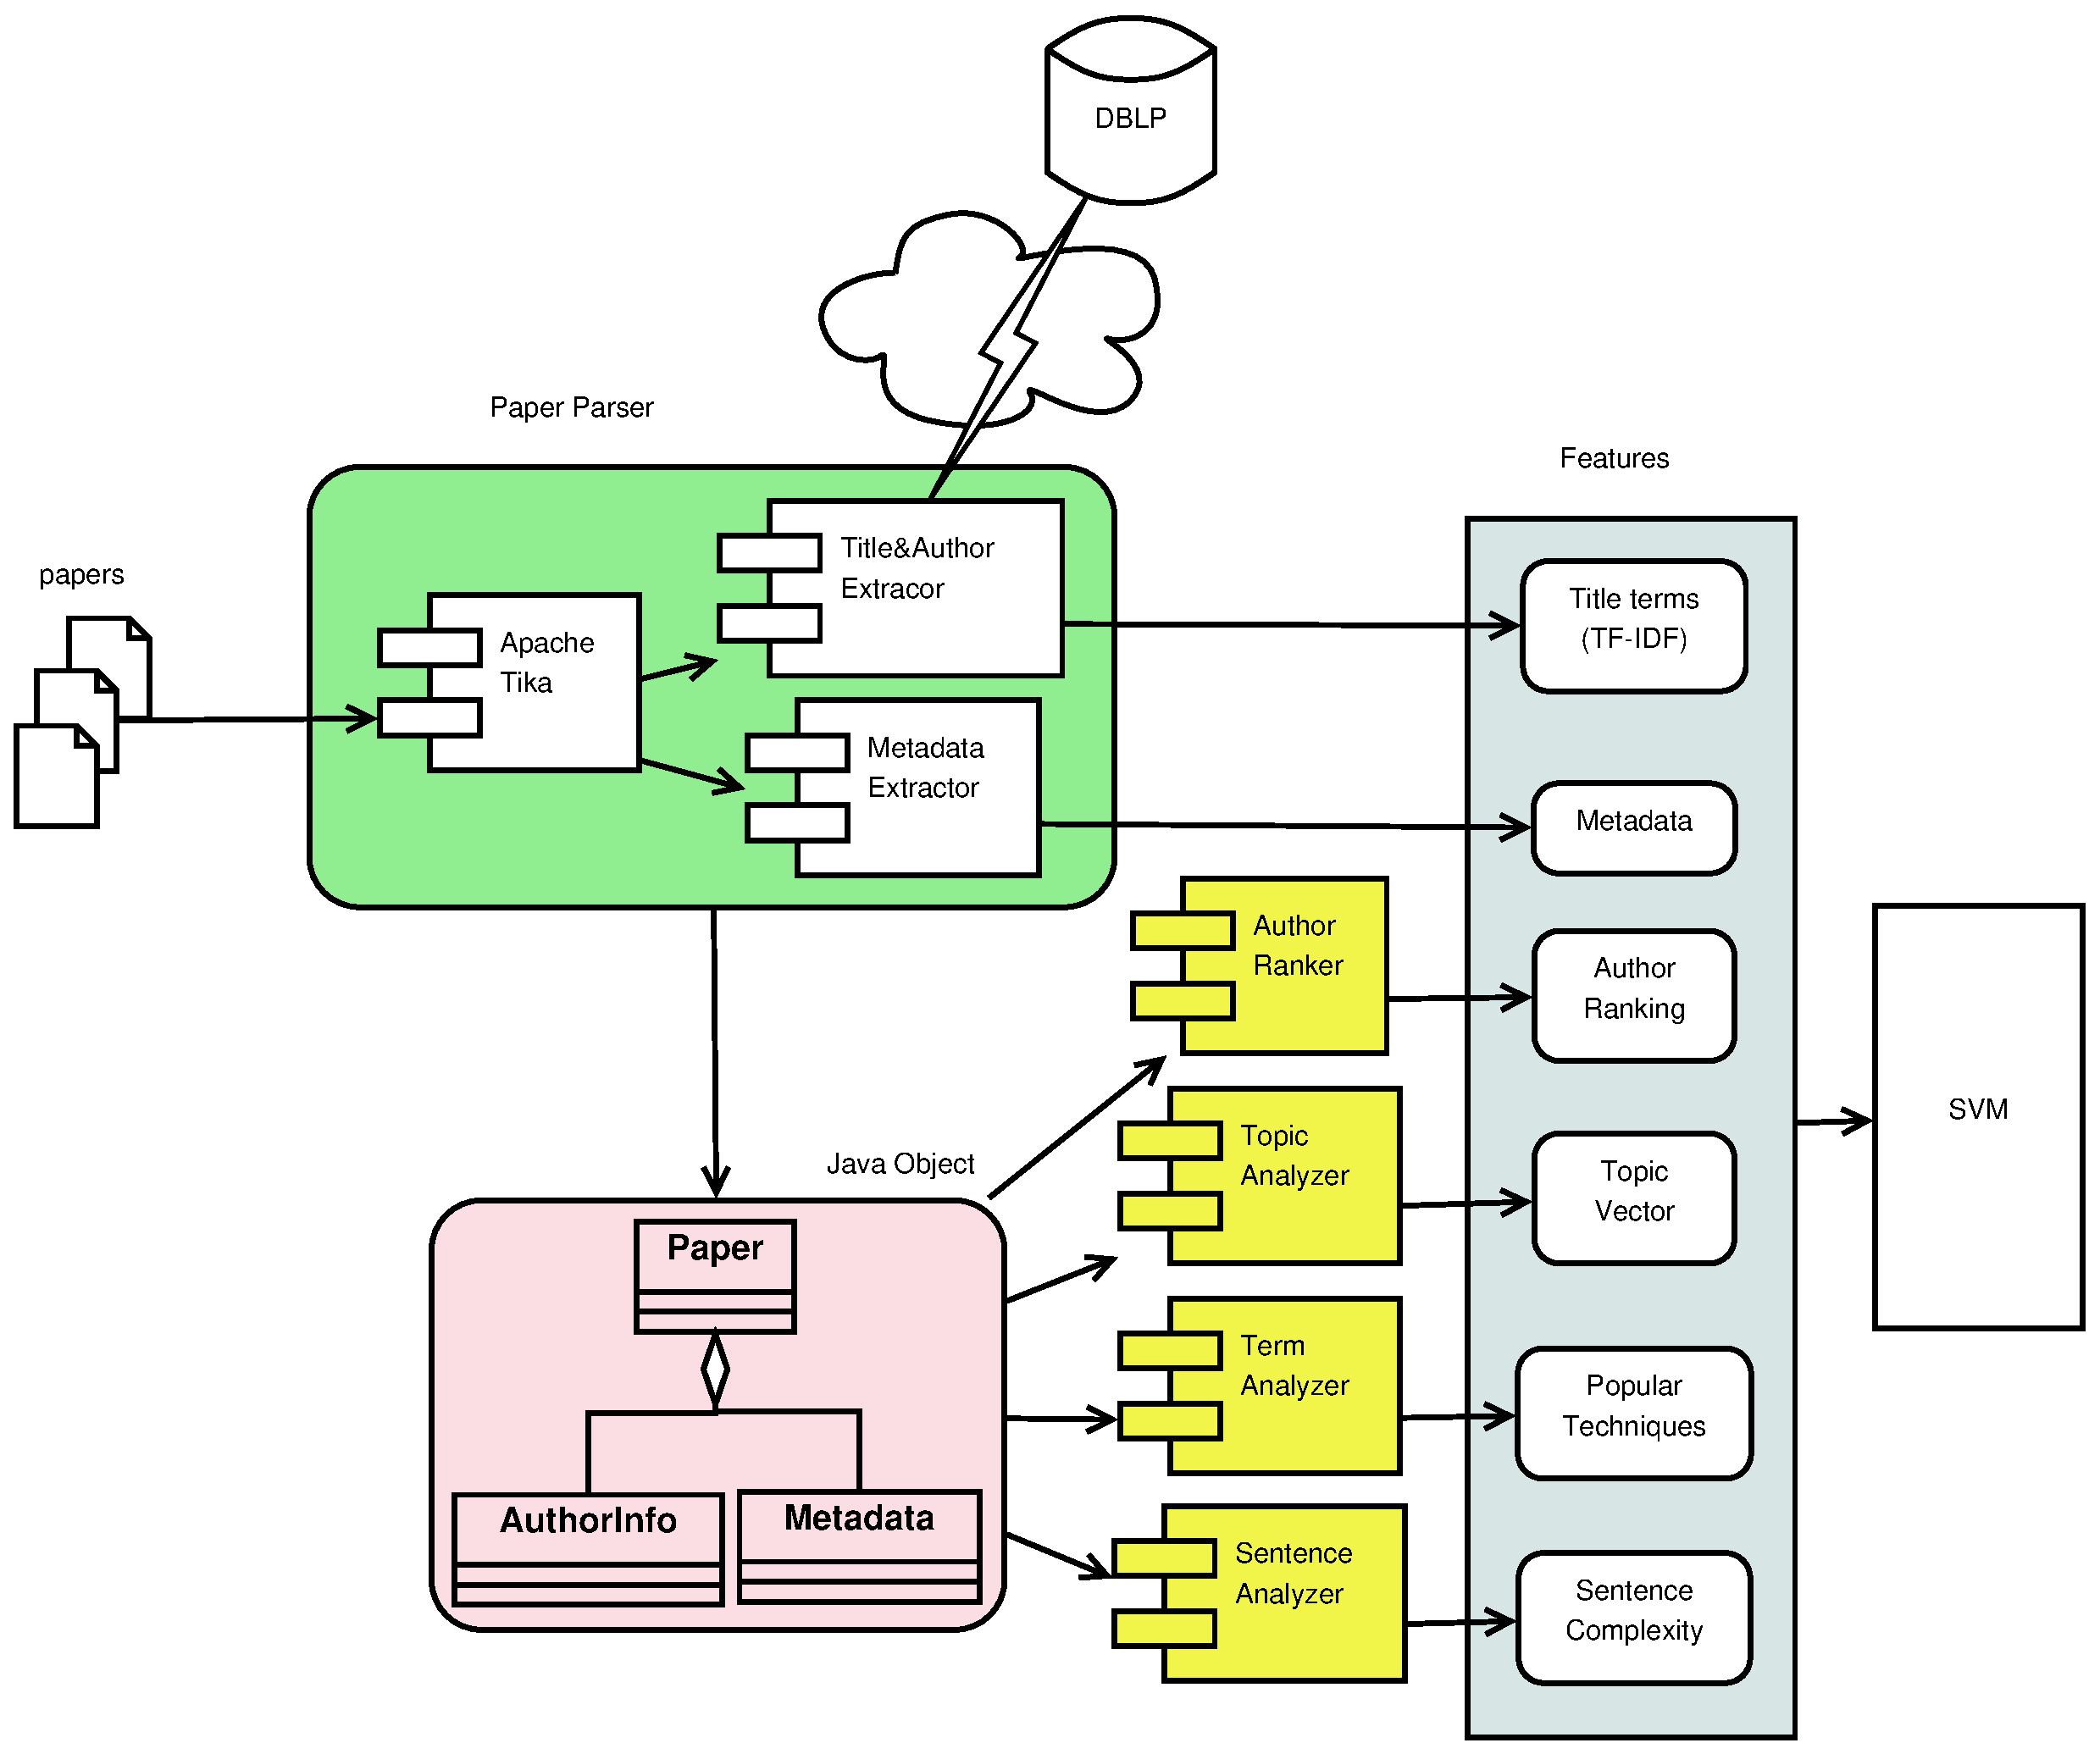
\includegraphics[width=0.7\textwidth]{materials/architecture.eps}
		\caption{The architecture of the proposed approach}
		\label{fig:architecture}
\end{figure*}
In this study, we first downloaded all the papers from ACL web-site. Then we send them to Automatic Reviewer. There are three main components in Automatic Reviewer: 1. paper parser; 2. feature extractors; and 3. model and evaluation component. 
The architecture is showed in Figure \ref{fig:architecture}.

Papers are first parsed into structured data (Java objects). Metadata from the paper are used directly as features. Then the parsed papers are processed by several feature extractors. Finally, the feature vectors are sent to Support Vector Machines (SVM) for model learning and evaluation.




\subsection{Paper parser}

There are three sub-components in the paper parser: Apache Tika [??], Metadata Extractor, and Title \& Author Extractor. 
Downloaded original papers are first sent to Apache Tika which is a PDF file parser. It can parse PDF file into HTML-like structured data. The paper is parsed into several <page> tags which contains <p> tags that denote the raw paragraphs in the original paper. 

Because the parsing is not very accuracy, the raw paragraphs contain all the texts in the paper, including the page foot, like “Proceedings of …”, “BioNLP 20...”. Those paragraphs are discarded. Then, the first raw paragraph is considered as the candidate title. The paragraph starts with “abstract” is the abstract paragraph. If there’s no paragraph starts with “abstract”, the first paragraph which contains more than 300 English letters is considered as abstract paragraph. 

We consider all the paragraphs between title and abstract as raw author info which contains author names, affiliations, and email addresses. All paragraphs after the key-word “reference” are considered as references. The other paragraphs between abstract and references are considered as content paragraphs. 

Content paragraphs are then sent to Metadata Extractor. 
Metadata Extractor uses regular expression \verb- "\^(fig\.|figure)\s*\d+"- and  \verb-"\^(tab\.|table)\s*\d+"- to match the figures and tables in each page. Continuous paragraphs which contain more than 30\% non- alphabet English letters are considered as one formula. These approaches may not be very accurate. However, since both training and testing papers are parsed based on this same rule, we think the inaccuracy is acceptable. Using the methods above, all the metadata are generated. 

Candidate title and raw author information are processed by Title \& Author Extractor. This extractor utilizes DBLP’s web service API: 
“http://www.dblp.org/search/api/?q=[TITLE]”  
where “[TITLE]” is the paper title to search. This API supports fuzzy query, so we send the raw title to the API and retrieve the most reliable one as the real title for the paper. Together with the title, author names are also returned from this API. Then the extractor uses regular express to match the email addresses within raw author info, the text between the author name and email addresses are considered as the author’s affiliation. 

Through the paper parser, the PDF paper is parsed into a Java “Paper” object. “Paper” contains one “Metadata”, several “Author” objects, and all sentences in each paragraph. The corresponding UML is attached in the Appendix. 


\subsection{Feature Extractors}
Besides the metadata feature which directly comes from parsed Metadata object, other features are generated by several feature extractors. 

•	Author ranker
Author ranker extracts the top 2000 authors in “Natural Language \& Speech” area from Microsoft Academic Search. Then the author names, affiliations and ranking are stored in a Lucene [??] index. Because there may be abbreviation in names which appeared in the paper, we send fuzzy query of author name to Lucene index to retrieve the ranking information. Also an empirical threshold value are set to filter those unlikely matching. 


•	Term analyzer
Term analyzer tries to catch concepts from paper at term-level. Right now the analyzer mainly focuses on the popular technique terms mentioned in the paper. Not like topic of paper, these technique terms concentrate on technique aspects of paper content. We manually created a list of technique terms and their synonyms and abbreviations. 

Term analyzer use this term table to generate a Boolean vector feature, each value in the vector corresponds to the existence of each technique term. 


•	Topic analyzer
We believe that during a period of time, some certain topics are more interested in a given research area, and those papers studied such topics have more chances been accepted by the conference in that research area. In order to find out what topics are more interested by the conference, we use LDA (Latent Dirichlet allocation) to extract 20 topics from all the training data. The probability distribution of the topics of paper is used as a feature vector.  

•	Sentence analyzer
Because there is a limitation of the number of pages in every conference, we think the sentence would be more complicated if the paper contains more information. Based on this assumption, we use sentence analyzer to analyze the complexities of sentences in each paper. The paragraphs in paper are first split into sentences, and then these sentences are parsed by Stanford Parser [??]. The entire parsing process is extremely slow. It costs more than 27 hours in our experiment machine (Intel Core i5, 2.27GHz, 6G RAM for JVM) with 5 working threads in parallel. After we got the parsed phrase structure tree from Stanford Parser, the depth of each sentence tree is used as the measurement of sentence complexity. 










\section{Results and Discussion}
We use the SVM with 10-fold-cross validation to evaluate our Automatic Reviewer system. The result of all positive predictions is used as the baseline. 


\subsection{Evaluation on Each Single Year Data}
As the first part of our experiment, 
we evaluate the proposed apporach the papers of each single year.
For each year of the years 2012, 2010 and 2007, 
we use 10-fold cross validation for the evaluation.



\subsection{Discussion and Conclusion} 

// may be changed according to new evaluation result
Form the result of evaluation, we can see that our model can predict whether a paper is accepted or not with good accuracy. The metadata and the topic distribution learned by LDA model are the best features. This result proved our assumption that certain topics are more favored by certain conference. Also, tables number is the best of all three metadata, which indicates that the reviewers of paper are more willing to see the well structured result of research rather than plain text. // TODO 

Features like popular techniques and author ranking do not work very good. This phenomena indicates that the quality of ACL conference is very high, the papers are thoroughly studied before accepting/rejecting, and the conference cares more about the content of paper rather than whether the techniques used are popular or not. Because the reviewing is blind, the author’s ranking cannot influence the decision of the reviewers. 

We find that our model seems work better on the more balanced dataset (i.e. the numbers of positive and negative samples are close to each other)

// TODO


In the future, we want to study how the topic/style of papers changes over the time. And we also want to extend our research to other conferences in other area. We want to find out the main difference between the accepted papers in different conferences, and different areas. 
Currently, the negative samples are workshop papers which may not be representative.  We are considering using papers come from lower-level conferences within the same research area as the negative samples. 



\begin{appendices}
\chapter{Additional materials}
\begin{figure*}[htb]
  \centering
	 	 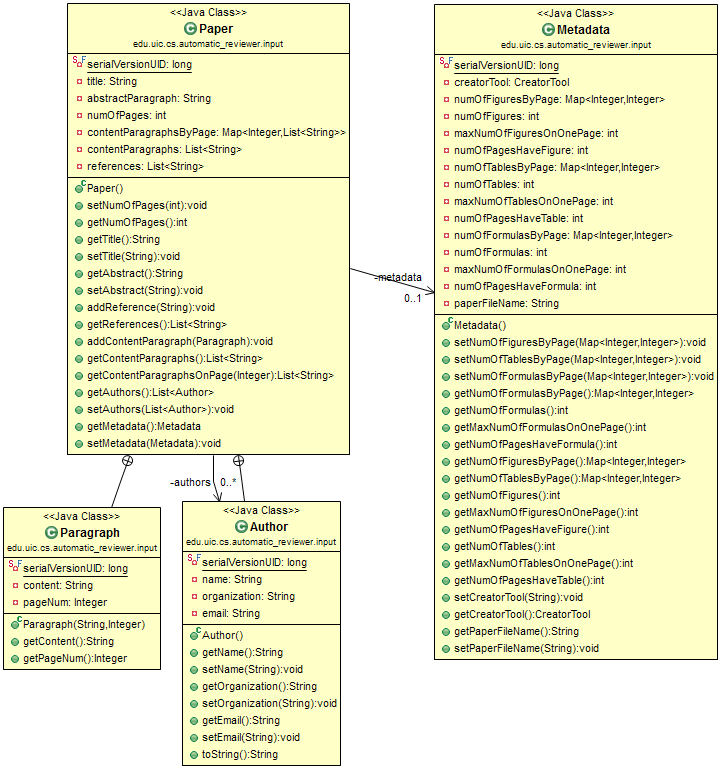
\includegraphics[width=0.7\textwidth]{materials/paper_uml.png}
		\caption{UML for the parsed Java Paper object}
		\label{fig:uml}
\end{figure*}



\chapter{Project Workload}
•	The blue parts are done by Hong Wang.
•	The red parts (including original paper gathering and evaluation) are done by Shuyang Lin.
•	This project report and previous presentation slides are done by both of them. 

\begin{figure*}[htb]
  \centering
	 	 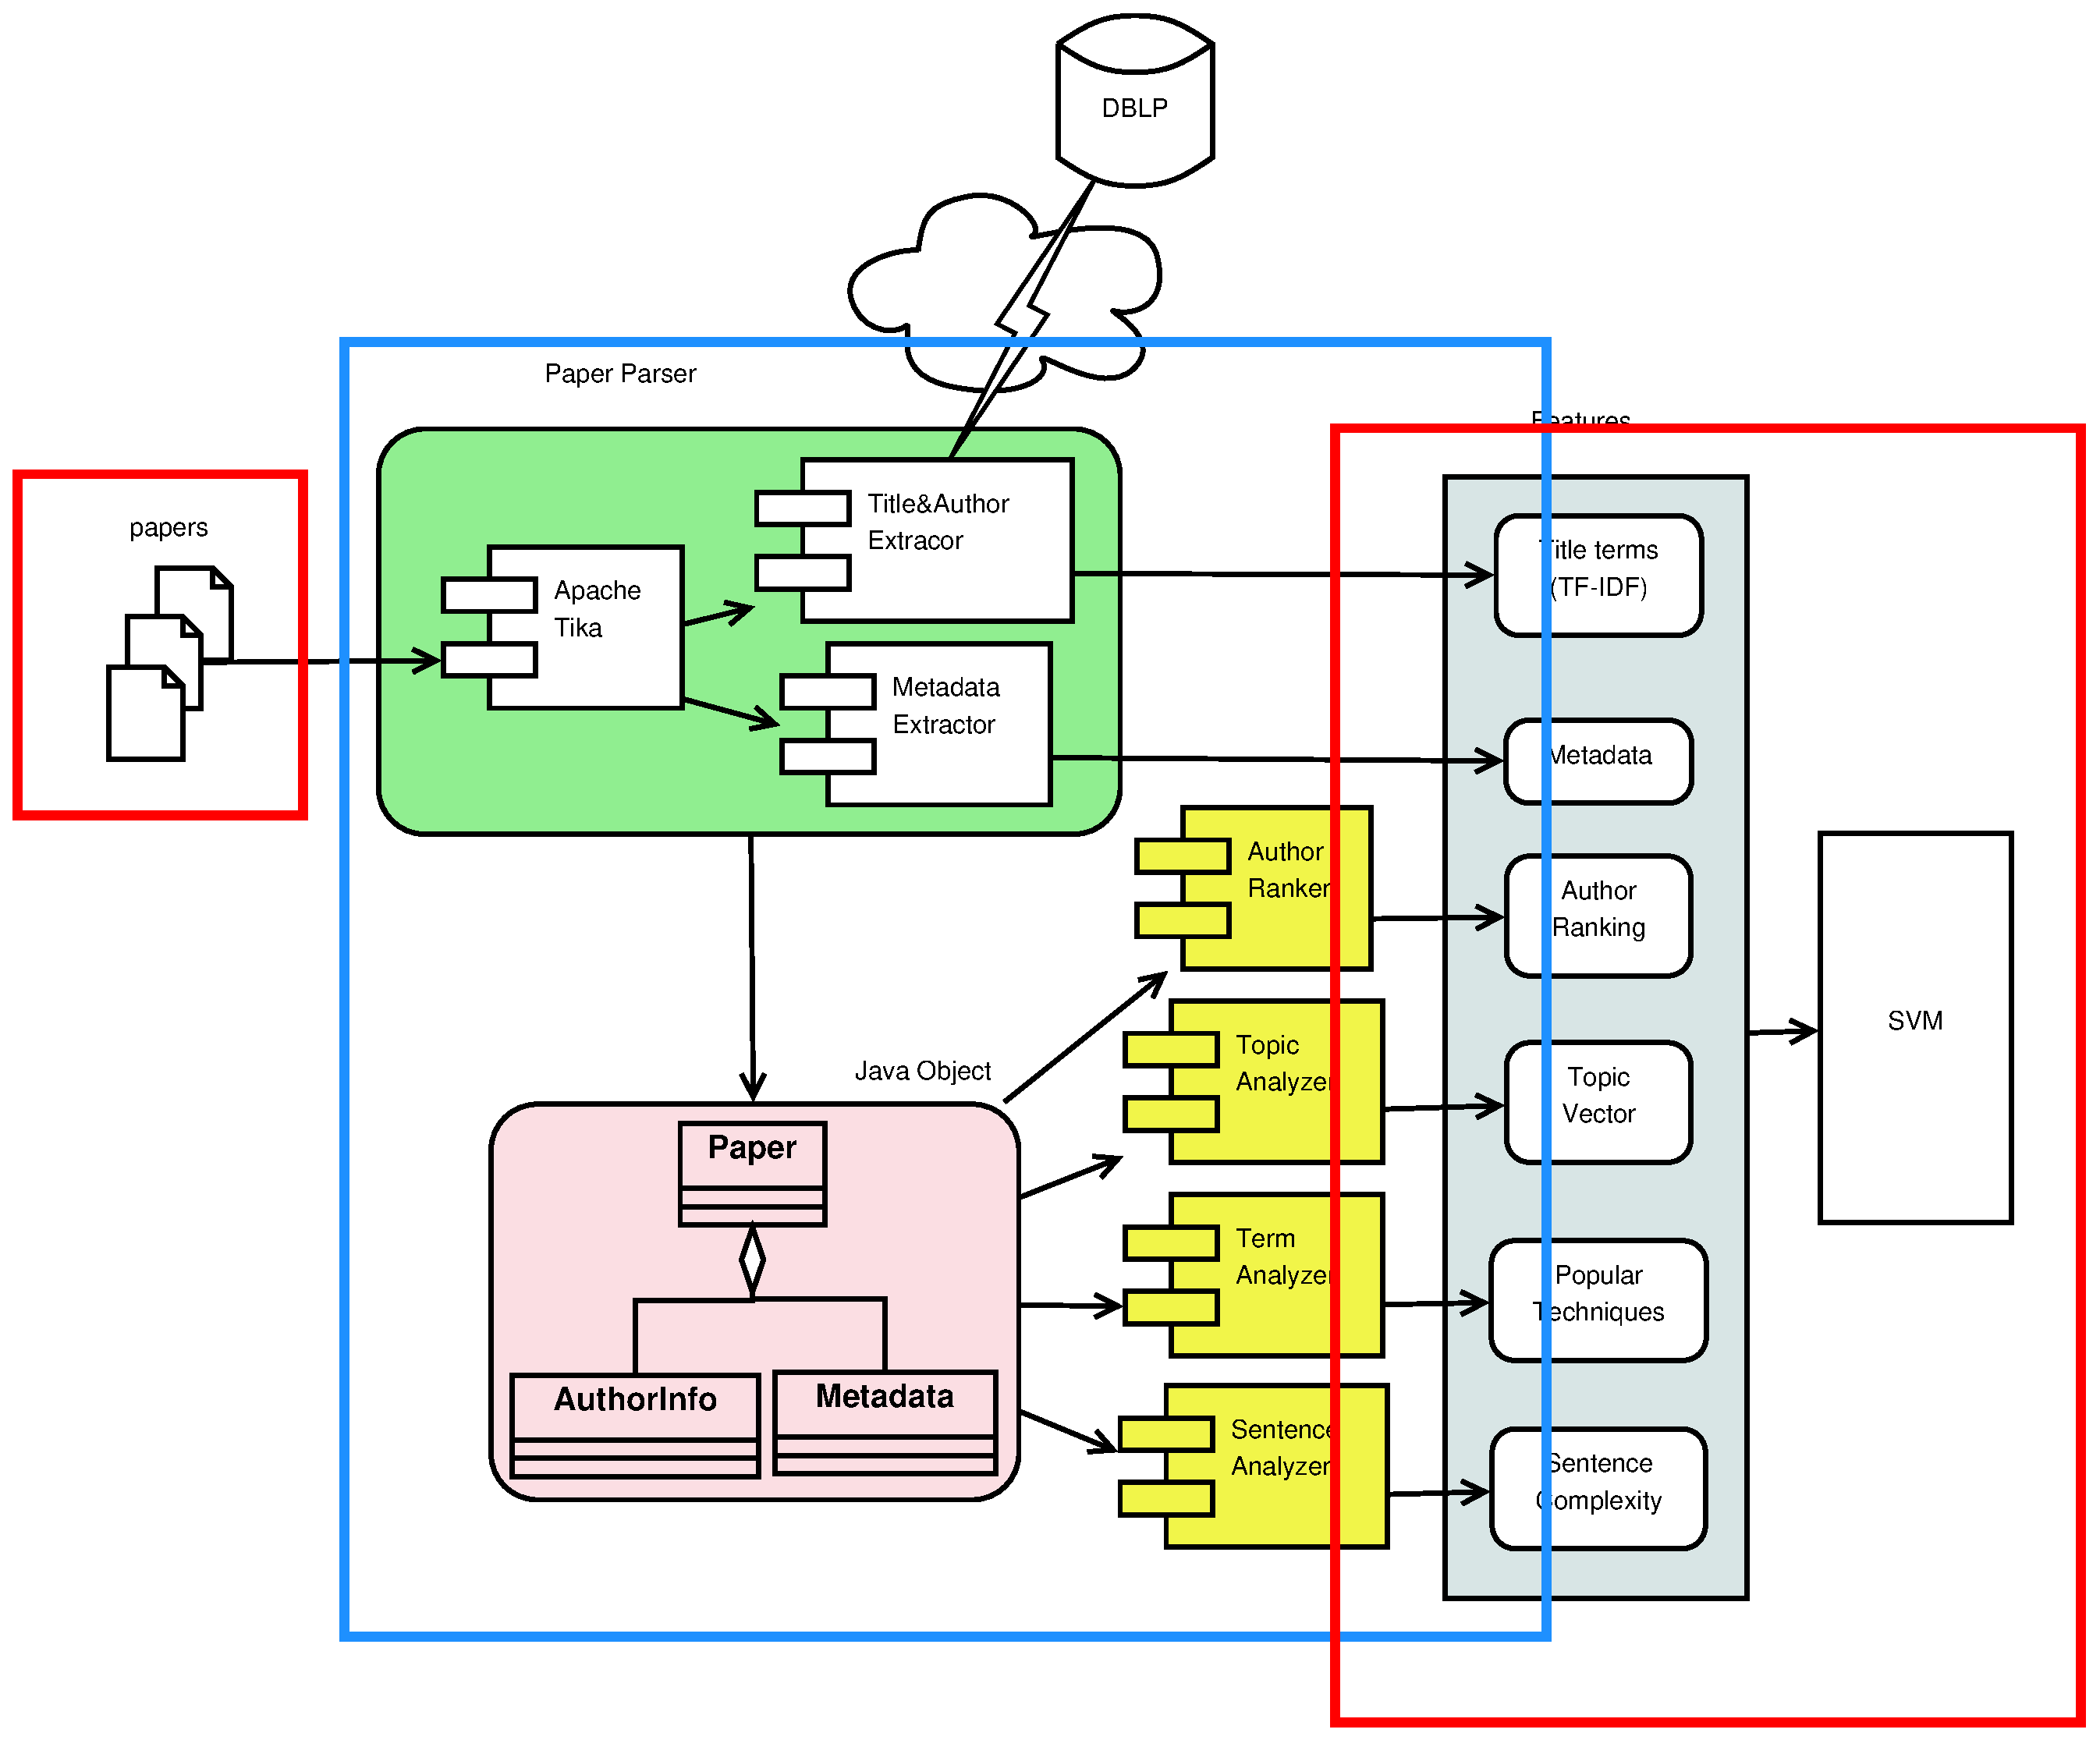
\includegraphics[width=0.5\textwidth]{materials/workload.eps}
		\caption{UML for the parsed Java Paper object}
		\label{fig:workload}
\end{figure*}



\end{appendices}



\end{document}

\section{Introduction}

The following instructions are directed to authors of papers accepted
for publication in the NAACL HLT 2013 proceedings.  All authors are required
to adhere to these specifications. Authors are required to provide 
a Portable Document Format (PDF) version of
their papers.  The proceedings will be printed on US-Letter paper.
Authors from countries in which access to word-processing systems is
limited should contact the publication chairs as soon as possible.

\paragraph{What's new} This year, grayscale readability will be enforced for all accepted
papers (\S\ref{ssec:accessibility}).  Apart from this, the style files and camera-ready requirements
are unchanged from last year.

\section{General Instructions}

Manuscripts must be in two-column format.  Exceptions to the
two-column format include the title, as well as the 
authors' names and complete
addresses (only in the final version, not in the version submitted for review), 
which must be centered at the top of the first page (see
the guidelines in Subsection~\ref{ssec:first}), and any full-width
figures or tables.  Type single-spaced.  Do not number the pages.
Start all pages directly under the top margin.  See the guidelines
later regarding formatting the first page.

%% If the paper is produced by a printer, make sure that the quality
%% of the output is dark enough to photocopy well.  It may be necessary
%% to have your laser printer adjusted for this purpose.  Papers that are too
%% faint to reproduce well may not be included.

%% {\bf Do not print page numbers on the manuscript.}  Write them lightly
%% on the back of each page in the upper left corner along with the
%% (first) author's name.

The maximum length of a manuscript is eight (8) pages for the main
conference, printed single-sided, plus two (2) pages for references
(see Section~\ref{sec:length} for additional information on the
maximum number of pages).  Do not number the pages.

The review process is double-blind, so do not include any author information (names, addresses) when submitting a paper for review.  However, you should allocate space for the names and addresses so that they will fit in the final (accepted) version.  This is best done by either providing fake or blank names and addresses (as shown in this paper).

\subsection{Electronically-available resources}

NAACL HLT provides this description in \LaTeX2e{} ({\tt naaclhlt2013.tex}) and PDF
format ({\tt naaclhlt2013.pdf}), along with the \LaTeX2e{} style file used to
format it ({\tt naaclhlt2013.sty}) and an ACL bibliography style ({\tt naaclhlt2013.bst}).
These files are all available at
{\tt http://naacl2013.naacl.org}.  A Microsoft Word
template file ({\tt naaclhlt2013.dot}) is also available at the same URL. We
strongly recommend the use of these style files, which have been
appropriately tailored for the NAACL HLT 2013 proceedings.


\subsection{Format of Electronic Manuscript}
\label{sect:pdf}

For the production of the electronic manuscript you must use Adobe's
Portable Document Format (PDF). This format can be generated from
postscript files: on Unix systems, you can use {\tt ps2pdf} for this
purpose; under Microsoft Windows, you can use Adobe's Distiller, or
if you have cygwin installed, you can use {\tt dvipdf} or
{\tt ps2pdf}.  Note 
that some word processing programs generate PDF which may not include
all the necessary fonts (esp. tree diagrams, symbols). When you print
or create the PDF file, there is usually an option in your printer
setup to include none, all or just non-standard fonts.  Please make
sure that you select the option of including ALL the fonts.  {\em
  Before sending it, test your {\/\em PDF} by printing it from a
  computer different from the one where it was created}. Moreover,
some word processor may generate very large postscript/PDF files,
where each page is rendered as an image. Such images may reproduce
poorly.  In this case, try alternative ways to obtain the postscript
and/or PDF.  One way on some systems is to install a driver for a
postscript printer, send your document to the printer specifying
``Output to a file'', then convert the file to PDF.

For reasons of uniformity, Adobe's {\bf Times Roman} font should be
used. In \LaTeX2e{} this is accomplished by putting

\begin{quote}
\begin{verbatim}
\usepackage{times}
\usepackage{latexsym}
\end{verbatim}
\end{quote}
in the preamble.

Additionally, it is of utmost importance to specify the {\bf
  US-Letter format} (8.5in $\times$ 11in) when formatting the paper.
When working with {\tt dvips}, for instance, one should specify {\tt
  -t letter}.

Print-outs of the PDF file on US-Letter paper should be identical to the
hardcopy version.  If you cannot meet the above requirements about the
production of your electronic submission, please contact the
publication chairs above  as soon as possible.


\subsection{Layout}
\label{ssec:layout}

Format manuscripts two columns to a page, in the manner these
instructions are formatted. The exact dimensions for a page on US-letter
paper are:

\begin{itemize}
\item Left and right margins: 1 inch
\item Top margin: 1 inch
\item Bottom margin: 1 inch
\item Column width: 3.15 inches
\item Column height: 9 inches
\item Gap between columns: 0.2 inches
\end{itemize}

\noindent Papers should not be submitted on any other paper size. Exceptionally,
authors for whom it is \emph{impossible} to format on US-Letter paper,
may format for \emph{A4} paper. In this case, they should keep the \emph{top}
and \emph{left} margins as given above, use the same column width,
height and gap, and modify the bottom and right margins as necessary.
Note that the text will no longer be centered.

\subsection{The First Page}
\label{ssec:first}

Center the title, author's name(s) and affiliation(s) across both
columns (or, in the case of initial submission, space for the names). 
Do not use footnotes for affiliations.  Do not include the
paper ID number assigned during the submission process. 
Use the two-column format only when you begin the abstract.

{\bf Title}: Place the title centered at the top of the first page, in
a 15 point bold font.  (For a complete guide to font sizes and styles, see Table~\ref{font-table}.)
Long title should be typed on two lines without
a blank line intervening. Approximately, put the title at 1in from the
top of the page, followed by a blank line, then the author's names(s),
and the affiliation on the following line.  Do not use only initials
for given names (middle initials are allowed). Do not format surnames
in all capitals (e.g., ``Bangalore,'' not ``BANGALORE'').  The affiliation should
contain the author's complete address, and if possible an electronic
mail address. Leave about 0.75in between the affiliation and the body
of the first page.

{\bf Abstract}: Type the abstract at the beginning of the first
column.  The width of the abstract text should be smaller than the
width of the columns for the text in the body of the paper by about
0.25in on each side.  Center the word {\bf Abstract} in a 12 point
bold font above the body of the abstract. The abstract should be a
concise summary of the general thesis and conclusions of the paper.
It should be no longer than 200 words.  The abstract text should be in 10 point font.

{\bf Text}: Begin typing the main body of the text immediately after
the abstract, observing the two-column format as shown in 
the present document.  Do not include page numbers.

{\bf Indent} when starting a new paragraph. For reasons of uniformity,
use Adobe's {\bf Times Roman} fonts, with 11 points for text and 
subsection headings, 12 points for section headings and 15 points for
the title.  If Times Roman is unavailable, use {\bf Computer Modern
  Roman} (\LaTeX2e{}'s default; see section \ref{sect:pdf} above).
Note that the latter is about 10\% less dense than Adobe's Times Roman
font.

\subsection{Sections}

{\bf Headings}: Type and label section and subsection headings in the
style shown on the present document.  Use numbered sections (Arabic
numerals) in order to facilitate cross references. Number subsections
with the section number and the subsection number separated by a dot,
in Arabic numerals. 

{\bf Citations}: Citations within the text appear
in parentheses as~\cite{Gusfield:97} or, if the author's name appears in
the text itself, as Gusfield~\shortcite{Gusfield:97}. In \LaTeX2e, the former is accomplished using
\verb|\cite| and the latter with \verb|\shortcite| or \verb|\newcite|.
Append lowercase letters to the year in cases of ambiguities.  
Treat double authors as in~\cite{Aho:72}, but write as 
in~\cite{Chandra:81} when more than two authors are involved. 
Collapse multiple citations as in~\cite{Gusfield:97,Aho:72}.

\textbf{References}: Gather the full set of references together under
the heading {\bf References}; place the section before any Appendices,
unless they contain references. Arrange the references alphabetically
by first author, rather than by order of occurrence in the text.
Provide as complete a citation as possible, using a consistent format,
such as the one for {\em Computational Linguistics\/} or the one in the 
{\em Publication Manual of the American 
Psychological Association\/}~\cite{APA:83}.  Use of full names for
authors rather than initials is preferred.  A list of abbreviations
for common computer science journals can be found in the ACM 
{\em Computing Reviews\/}~\cite{ACM:83}.

The \LaTeX{} and Bib\TeX{} style files provided roughly fit the
American Psychological Association format, allowing regular citations, 
short citations and multiple citations as described above.

{\bf Appendices}: Appendices, if any, directly follow the text and the
references (but see above).  Letter them in sequence and provide an
informative title: {\bf Appendix A. Title of Appendix}.

\textbf{Acknowledgment} sections should go as a last (unnumbered) section immediately
before the references.  

\subsection{Footnotes}

{\bf Footnotes}: Put footnotes at the bottom of the page. They may
be numbered or referred to by asterisks or other
symbols.\footnote{This is how a footnote should appear.} Footnotes
should be separated from the text by a line.\footnote{Note the
line separating the footnotes from the text.}  Footnotes should be in 9 point font.

\subsection{Graphics}

{\bf Illustrations}: Place figures, tables, and photographs in the
paper near where they are first discussed, rather than at the end, if
possible.  Wide illustrations may run across both columns and should be placed at
the top of a page. Color illustrations are discouraged, unless you have verified that 
they will be understandable when printed in black ink. 

\begin{table}
\begin{center}
\begin{tabular}{|l|rl|}
\hline \bf Type of Text & \bf Font Size & \bf Style \\ \hline
paper title & 15 pt & bold \\
author names & 12 pt & bold \\
author affiliation & 12 pt & \\
the word ``Abstract'' & 12 pt & bold \\
section titles & 12 pt & bold \\
document text & 11 pt  &\\
abstract text & 10 pt & \\
captions & 10 pt & \\
bibliography & 10 pt & \\
footnotes & 9 pt & \\
\hline
\end{tabular}
\end{center}
\caption{\label{font-table} Font guide. }
\end{table}

{\bf Captions}: Provide a caption for every illustration; number each one
sequentially in the form:  ``Figure 1. Caption of the Figure.'' ``Table 1.
Caption of the Table.''  Type the captions of the figures and 
tables below the body, using 10 point text.  

\subsection{Accessibility}
\label{ssec:accessibility}

In an effort to accommodate the color-blind (as well as those printing to paper), grayscale
readability for all accepted papers will be enforced.  Color is not forbidden, but authors should
ensure that tables and figures do not rely solely on color to convey critical distinctions.

\section{Length of Submission}
\label{sec:length}

The NAACL HLT 2013 main conference accepts submissions of long papers
and short papers.  The maximum length of a long paper manuscript is
eight (8) pages of content and two (2) additional pages of references
\emph{only} (appendices count against the eight pages, not the
additional two pages).  The maximum length of a short paper manuscript
is four (4) pages and two (2) additional pages of references.  For
both long and short papers, all illustrations, references, and
appendices must be accommodated within these page limits, observing
the formatting instructions given in the present document.  Papers
that do not conform to the specified length and formatting
requirements are subject to be rejected without review.

\section{Double-blind review process}
\label{sec:blind}

As the reviewing will be blind, the paper must not include the authors' names and affiliations. Furthermore, self-references that reveal the author's identity, e.g., ``We previously showed (Smith, 1991) ...'' must be avoided. Instead, use citations such as ``Smith previously showed (Smith, 1991) ...'' Papers that do not conform to these requirements will be rejected without review. In addition, please do not post your submissions on the web until after the review process is complete.

\section*{Acknowledgments}

Do not number the acknowledgment section.

\begin{thebibliography}{}

\bibitem[\protect\citename{Aho and Ullman}1972]{Aho:72}
Alfred~V. Aho and Jeffrey~D. Ullman.
\newblock 1972.
\newblock {\em The Theory of Parsing, Translation and Compiling}, volume~1.
\newblock Prentice-{Hall}, Englewood Cliffs, NJ.

\bibitem[\protect\citename{{American Psychological Association}}1983]{APA:83}
{American Psychological Association}.
\newblock 1983.
\newblock {\em Publications Manual}.
\newblock American Psychological Association, Washington, DC.

\bibitem[\protect\citename{{Association for Computing Machinery}}1983]{ACM:83}
{Association for Computing Machinery}.
\newblock 1983.
\newblock {\em Computing Reviews}, 24(11):503--512.

\bibitem[\protect\citename{Chandra \bgroup et al.\egroup }1981]{Chandra:81}
Ashok~K. Chandra, Dexter~C. Kozen, and Larry~J. Stockmeyer.
\newblock 1981.
\newblock Alternation.
\newblock {\em Journal of the Association for Computing Machinery},
  28(1):114--133.

\bibitem[\protect\citename{Gusfield}1997]{Gusfield:97}
Dan Gusfield.
\newblock 1997.
\newblock {\em Algorithms on Strings, Trees and Sequences}.
\newblock Cambridge University Press, Cambridge, UK.

\end{thebibliography}

\end{document}
